
\chapter{Certified Programming}
\label{chap:certprog}

The Alba programming languages makes certain guarantees.
\begin{enumerate}
\item A program cannot crash.

\item There are no endless loops (i.e. the program cannot not freeze).

\item All functions perform according to their specification.
\end{enumerate}

The first point is achieved by a strict typing, a strict handling of pattern
match (all cases must be handled) and the lack of an undisciplined exception
processing. An undisciplined exception processing would be to allow the
throwing of exceptions without enforcement of the handling of exceptional
conditions.

The second point (no endless loops) is achieved by basing all recursions on
some argument which is decreased at each recursive call. This guarantees that
all functions must terminate.

The third point is achieved by implementing the curry howard isomorphism in
the form of propositions as types. It is possible to encode propositions like
$i > 0$ as a type and writing functions which return an inhabitant of these
types i.e. functions which generate a proof of the proposition.

Having this tool, it is possible to state some properties of functions and
prove these properties by writing functions which return proofs of the
desired properties.

In Alba a proof is just a functional programm. A proof of the implication $a
\imp b$ is a function which maps a proof of the proposition $a$ into a proof
of the proposition $b$.

Proofs in Alba are normal objects with the difference that these proof objects
do not exist at runtime. But they are data, which can be arguments to
functions. The functions can iterate over the proof data and can generate
other proof objects.

The purpose of this chapter is to demonstrate the possibility in Alba to write
functions and prove properties about these functions in the same language.




\newpage
\section{Logic}
\label{sec:certprog-logic}


In this chapter we use functional programming to prove some basic laws of
logic. The Alba compiler \emph{knows} how to handle propositions and is able
to do all the proofs in this chapter automatically. You are never required to
produce such proofs by hand.

But is very instructive to see how proofs of these basic laws of logic can be
generated by using functional programming. Therefore we give manual proofs
here.



\subsection{Ex Falso}

\emph{Ex falso quodlibet} i.e. from a false (or contradictory) assumption you
can conclude anything, is a basic law of logic. It is possible to prove this
law in Alba by writing a function with the signature

\begin{alba}
    exFalso (A: Any): false -> A := ...
\end{alba}
%
The signature of this function gives the promise: \emph{Give me an arbitrary
type and a proof of \code{false} and I return you an object of that type}. Since
\code{a:Proposition} implies \code{a:Any} in Alba, all propositions can be
entered as actual arguments for \code{A}.


Remember that \code{false} is an inductive type with the following definition.
\begin{alba}
    class false: Proposition := -- no constructors
\end{alba}
%
Since there are no constructors we can complete the desired function

\begin{alba}
    exFalso (A: Any): false -> A :=
        case
            -- empty pattern match, because there are no constructors
\end{alba}
%
Each case must return an object of the desired type. But since there are no
cases, there is nothing to be done.






\subsection{Negation}

Negation is defined in the prelude as
\begin{alba}
  (not) (a: Proposition): Proposition :=
    a => false
\end{alba}

We want to prove the contrapositive law of logic which states
\begin{alba}
  (a => b) => (not b => not a)
\end{alba}
for all propositions \code{a} and \code{b}. A proof of that fact would be
written in Alba as the function
%
\begin{alba}
  contrapositive (a b: Proposition): (a => b) => not b => not a
  :=
    _      -- '_' means: Compiler, please generate a proof!
\end{alba}
%
It is not necessary to write such a proof by hand, because the compiler can
generate such a proof automatically. But if you want to write the proof
explicitly it looks like

\begin{alba}
    contrapositive (a b: Proposition): (a => b) => not b => not a
    :=
        \ fab notB evA := fab evA |> notB
\end{alba}

\noindent Explanation: A proof of \code{not a} is a function which maps a proof
of \code{a} into a proof of false. If we have a proof of \code{a} we can use the
argument \code{fab} which maps a proof of \code{a} into proof of
\code{b} and then use \code{notB} which maps a proof of \code{b} into a proof
of \code{false} which is the desired result.



Note that in classical logic the two propositions
\begin{alba}
  a  =>  b

  not b => not a
\end{alba}
%
are equivalent. This is not the case in constructive logic on which Alba is
based. Suppose we wanted to prove
%
\begin{alba}
  (not b => not a) => a => b
\end{alba}
%
in Alba. In order to do this we need a function
\begin{alba}
  contra2 a b (p: not b => not a) (pa: a): b :=
     ...
\end{alba}
%
It is not difficult to see that there is no way to generate a proof of \code{b}
by using the arguments. The second argument of the function is atomic i.e. it
is not a function which can be applied. The first argument is a function whose
type we can expand to get
\begin{alba}
  p: (b => false) => a => false
\end{alba}
%
\code{p} is a function with two arguments. There is no way to supply the first
argument. Therefore we cannot use \code{p} and have no possibility to return
an expression of type \code{b}.


However there is a double negation correspondence between classical and
constructive logic. Whenever classical logic is capable to prove \code{a},
constructive logic is capable to prove \code{not not a}. I.e. we should be able
to prove

\begin{alba}
  (not b => not a) => a => not not b
\end{alba}
and define a function with the signature

\begin{alba}
  contra3 (a b: Propositon): (not b => not a) => a => not not b :=
    ...
\end{alba}

Now we have more possibilities because we are no longer required to prove
\code{b} directly, but only to derive \code{false} from \code{not b}. This
opens the possibility to use the function of type \code{not b => not a}.
%
\begin{alba}
    contra3 (a b: Proposition): (not b => not a) => a => not not b
    :=
        \   fNotBNotA evA notB: false :=
                fNotBNotA notB evA
\end{alba}






\subsection{Disjunction}

Logical disjunction is defined in the prelude as the inductive type
%
\begin{alba}
    class
        (or) (a b: Proposition): Proposition
    :=
        left:  a => a or b
        right: b => a or b
\end{alba}
%
i.e. you can either use a proof of \code{a} or a proof of \code{b} to generate
a proof of \code{a or b}.

It is a basic law of logic that \code{a or b} and \code{b or a} are
equivalent, i.e. we should be able to prove
%
\begin{alba}
  a or b  =>  b or a
\end{alba}
%
We prove this fact by defining the corresponding function which pattern
matches on the construction of \code{a or b}
%
\begin{alba}
    swapOr (a b: Proposition): a or b => b or a
    :=
        case
            left pa  := right pa
            right pb := left pb
\end{alba}

\noindent Another law of logic states
\begin{alba}
  a or b  =>  (a => c) => (b => c)  =>  c
\end{alba}
%
i.e. whenever we have a prove of \code{a or b} and are able to conclude
\code{c} from \code{a} and \code{c} from \code{b}, then we are able to
conclude \code{c}.

A function which proves this fact is easy to implement by pattern matching on
the construction of \code{a or b}.

\begin{alba}
    eliminateOr
        (a b c: Proposition)
        :   a or b
            => (a => c)
            => (b => c)
            => c
    :=
        case
            left pa :=
                \ fac _ := fac pa

            right pb :=
                \ _ fbc := fbc pb
\end{alba}










\subsection{Conjunction}

\begin{alba}
    class
        (and) (a b: Proposition): Proposition
    :=
        (,): a => b => a and b
\end{alba}


\begin{alba}
    swapAnd (a b: Proposition): a and b => b and a
    :=
        case
            (pa, pb) := (pb, pa)
\end{alba}


\begin{alba}
    eliminate1And (a b: Proposition): a and b => a :=
        case
            (pa, pb) := pa
\end{alba}








\vskip 5mm
\subsection{De Morgan's Laws}

The De Morgan's Laws are other basic laws of logic. The first of the De
Morgan's laws states the equivalence of the two statements
\begin{alba}
  not (a or b)

  not a and not b
\end{alba}
%
In order to prove the equivalence we have to prove both directions.
\begin{alba}
    deMorgan1Forward
        (a b: Proposition)
        : not (a or b) => not a and not b
    :=
        \ notAOrB :=
            (left >> notAOrB,  right >> notAOrB)
\end{alba}
%
Explanation: \code{notAOrB} is a function which maps evidence of \code{a or b}
into evidence of \code{false}. A proof of \code{not a} needs a function which
maps evidence of \code{a} into evidence of \code{false}. Therefore we can
combine \code{left} which maps evidence of \code{a} into evidence of \code{a or
b} and \code{notAOrB} which maps evidence of \code{a or b} into evidence of
\code{false} and we are done for \code{not a}. The proof of \code{not b} follows
the same pattern.



\begin{alba}
    deMorgan1Backward
        (a b: Proposition)
        : not a and not b => not (a or b)
    :=
        case
            (notA, notB) :=
                case
                    left evA :=
                        notA evA
                    right evB :=
                        notB evB
\end{alba}


There is a second De Morgan's law stating the equivalence of
\begin{alba}
  not a or not b

  not (a and b)
\end{alba}

The forward direction can be proved by the function
\begin{alba}
    deMorgan2Forward
        (a b: Proposition)
        : not a or not b => not (a and b)
    :=
        case
            left notA :=
                case
                    (evA, _) :=
                        notA evA
            right notB :=
                case
                    (_, evB) :=
                        notB evB
\end{alba}


In trying to prove the backward direction we face some difficulties. In order
to prove \code{not a or not b} we have to prove either \code{not a} or
\code{not b}. The only premise we have is \code{not (a and b)} which is a
function mapping any proof of \code{a and b} into \code{false}.

This proof is not possible in constructive logic. Therefore it is not possible
to prove it in Alba either.

In order to prove a disjunction in constructive logic we have to decide which
of the two possibilities of \code{not a or not b} we want to prove. There is
no possibility to make such a decision by looking only at \code{not (a and
  b)}.











\subsection{Existential Quantification}

The existence of an object with a certain property is expressed in Alba by the
inductive type
%
\begin{alba}
    class
        exist A (f: Predicate A): Proposition
    create
        witness x: f x -> exist f
\end{alba}
%
i.e. the existence of an object with a certain property is proved by providing
a witness and a proof that the witness satisfies the required property.

In Alba we write
%
\begin{alba}
  some (x:A): f x

  -- or

  some x: f x   -- if the type 'A' can be inferred from the context
\end{alba}
%
as another way to express the proposition
%
\begin{alba}
  exist f
\end{alba}

A basic law of logic states
%
\begin{alba}
  (some x: f x) => (all x: f x => a) => a
\end{alba}
%
Proofs using this law reads like
\begin{quote}
  We know that there exists an object satisfying $f$. Let $x$ be such an
  object satisfying $f$. From $ f x$ we can conclude $a$. Therefore $a$ is
  valid.
\end{quote}

We can prove this law in Alba by writing the function
\begin{alba}
    exist_elim
        (A: Any)
        (f: Predicate A)
        (prop: Proposition)
        : some x: f x => (all x: f x => prop) => prop
    :=
        \   some_x
            allx
        :=
            inspect some_x case
                witness x fx :=
                    allx x fx
\end{alba}


Like for logical disjunction and conjunction there are two De Morgan's laws for
existential and universal quantification. The first law states the equivalence
of
\begin{alba}
  not (some x: f x)

  all x: not (f x)
\end{alba}
or in words
\begin{quote}
  If there are no objects satisfying a certain property, then all objects do
  not satisfy the property. And if all objects do not satisfy a propert, then
  there are no objects satisfying the property.
\end{quote}

The proofs of the forward and backward direction are not complicated.

\begin{alba}
    ex_de_morgan1_forward
        (A: Any)
        (f: Predicate A)
        : not (some x: f x) => all x: not (f x)
    :=
        \   no_x
            x
            fx
        :=
            no_x (witness x fx)
\end{alba}


\begin{alba}
    ex_de_morgan1_backward
        (A: Any)
        (f: Predicate A)
        : (all x: not (f x)) => not (some x: f x)
    :=
        \   all_not
            some_x
        :=
            inspect some_x case
                witness x fx :=
                    all_not x fx
\end{alba}

The second De Morgan's law states the equivalence of
\begin{alba}
  some x: not (f x)

  not all x: f x
\end{alba}

The forward direction is easy.

\begin{alba}
    ex_de_morgan2_forward
        (A: Any)
        (f: Predicate A)
        : (some x: not (f x)) => not (all x: f x)
    :=
        \   some_x
            all_x
        :=
            inspect some_x case
                witness x not_fx :=
                    not_fx (all_x x)
\end{alba}

However the backward direction is not possible to prove. Constructive logic
requires us to find a witness in order to prove
\begin{alba}
  some x: not (f x)
\end{alba}
%
But the premise
%
\begin{alba}
  not all x: f x
\end{alba}
does not give us any possibility to extract a witness which does not satisfy
the property \code{f}










%-----------------------------------
\section{Specified Types}
%-----------------------------------

In the previous section we defined a function \code{reverse\_prepend} which
should reverse a list and prepend it in front of another list. In a second
step we proved that the function does the expected.

This signals that we might be able to use a specified type (i.e. a type whose
inhabitants satisfy a specification) as a result and implement the function
and the proof of its specification hand in hand.

A specified type is an inductive type of the form
%
\begin{alba}
   class Specified A (f: Predicate A): Any create
     specified x: f x -> Specified f
\end{alba}

The type \code{Specified} is known to the compiler and instead of writing
%
\begin{alba}
  Specified (\ (x:T) := exp)
\end{alba}
%
we can use syntactic sugar and write
%
\begin{alba}
  {x: T : exp}
  -- or
  {x: exp}     -- if the type 'T' can be inferred from the context.
\end{alba}


If we use a specified type in \code{reverse\_prepend} we get the signature
\begin{alba}
  reverse_prepend A (a b: List A): {c: c = a.reverse + b} :=
    ...
\end{alba}

Any implementation of \code{reverse\_prepend} must satisfy the specification
i.e. it has to return a list \code{c} which satisfies
\begin{alba}
  c = a.reverse + b
\end{alba}


The implementation of the function includes the proof of the specification.

\begin{alba}
  reverse_prepend A (a b: List A): {c: c = a.reverse + b} :=
    inspect a case
      [] :=
        specified b where
          _: b = [].reverse + b := _

      h ^ t :=
        inspect t.reverse_prepend (h ^ b) case
          specified c :=
            specified c where
              _: c = (h ^ t).reverse + b :=
                via t.reverse + (h ^ b)      -- hypo
                    t.reverse + ([h] + b)    -- def '+'
                    t.reverse + [h] + b      -- '+' assoc
                    (h ^ t).reverse + b      -- def 'reverse'
\end{alba}


Since the Alba compiler \emph{knows} the mechanics of a specified type, we can
omit one pattern match.

\begin{alba}
  reverse_prepend A (a b: List A): {c: c = a.reverse + b} :=
    inspect a case
      [] :=
        specified b

      h ^ t :=
        t.reverse_prepend (h ^ b) where
          _ c (p: c = t.reverse + (h ^ b))
            : c = (h ^ t).reverse + b :=
             via t.reverse + (h ^ b)      -- 'p'
                 t.reverse + ([h] + b)    -- def '+'
                 t.reverse + [h] + b      -- '+' assoc
                 (h ^ t).reverse + b      -- def 'reverse'
\end{alba}

In this definition we give the compiler a hint on how to transform a proof of
the specification of the recursive call into a proof of the specification of
the outer call.

In the runtime all specifications and proofs are erased. Therefore the
definition of the function \code{reverse\_prepend} in this chapter and the
previous chapter are identical in the runtime.








%-----------------------------------
\section{Equality}
%-----------------------------------



\subsection{Definition and Properties}

Equality is defined in Alba as an inductive type.
\begin{alba}
    class
        (=) (A: Any) (a: A): Predicate A
            -- Note: 'Predicate A' expands to
            --       'A -> Proposition'
    :=
        identical: a = a
\end{alba}

Note that the type \code{A} and the object \code{a} are parameters of the
inductive type. The expression \code{(=) a} is a predicate i.e. a function
\code{\textbackslash\ x := a = x} mapping each object \code{x} into the
proposition \code{a = x}.

In the proposition \code{a = b} the character of the left argument \code{a} and
the right argument \code{b} is different. The first argument is a parameter and
the second argument is an index.

A pattern match on an equality of the form \code{a = b} needs two arguments. The
first argument is an expression for \code{b} and a proof of \code{a = b}. A
pattern match has a dependent type.

\begin{alba}
    (case identical a := ...)
    : all b: a = b => goal

    -- 'b' usually occurs in 'goal'
\end{alba}

An inspect expression needs the two arguments as well
%
\begin{alba}
    inspect
        b; aEQb
    case
        identical a := ...
\end{alba}
%
which the compiler desugars to
\begin{alba}
    (case
        identical a := ...
    )
        b aEQb
\end{alba}



It is easy to prove the symmetry of equality by using a pattern match.
\begin{alba}
    symmetric
        (A: Any) (a: A)
        : all b: a = b => b = a
    :=
        -- Elimination function
        -- \ b (p: a = b) := b = a
        case
            identical a :=
                    -- goal: a = a
                identical a
\end{alba}

In the same manner the transitivity of equality can be proved.
\begin{alba}
    transitive
        (A: Any) (a b c: A)
        : a = b => b = c => a = c
    :=
        \ aEQb :=
            inspect
                b aEQb
            case
                -- Elimination function
                -- \ b (p: a = b) := b = c => a = c
                identical a :=
                        -- goal a = c => a = c
                    identity
\end{alba}
%
Note that the compiler needs the index argument as a variable in order to see
how the goal depends on that variable. In the pattern match it substitutes the
index variable \code{b} in the goal by the parameter \code{a}.

\noindent The desugared form with explicit result type looks like
\begin{alba}
    transitive
        (A: Any) (a b c: A)
        : a = b => b = c => a = c
    :=
        \ aEQb :=
            (
                case
                    identical a := identity
                : all b: a = b => b = c => a = c
            )
                b
                aEQb
\end{alba}



\subsection{Leibniz Equality}

Equality defined with the above inductive type is a rather strong
property. This kind of equality is also known as \emph{Leibniz equality} which
means that two equal objects satisfy the same properties.
%
\begin{alba}
    leibniz
        (A: Any)
        (f: Predicate A)
        (a b: A)
        : a = b => f a => f b
    :=
        ...
\end{alba}


We can prove this theorem by a pattern match on the proof of the equality.

\begin{alba}
    leibniz
        (A: Any)
        (f: Predicate A)
        (a: A)
        : all b: a = b => f a => f b
    :=
        case
            -- Elimination function
            -- \ b (p: a = b) := f a => f b
            identical a:=
                -- goal f a => f a
                identity
\end{alba}


In order to see why the proof is correct we have added the elimination function
into the pattern match expression. The arguments of an elimination function are
the indices of the inductive type and an object of the inductive type. The index
of \code{a = b} is \code{b} and the object of the inductive type is \code{eq}.

If we apply the elimination function to the two arguments \code{b} and
\code{eq}, we get the required result type \code{f a => f b} of the pattern
match expression. This shows that the elimination function is correct.

Note that the only constructor \code{identical} constructs \code{a = a}, i.e.
the index is \code{a}. Therefore the expression on the right side of the case
must construct an object of type \code{f a}.



\subsection{Argument Equality}

\begin{alba}
    apply
        (A B: Any) {a b: A}
        (f: A -> B)
        (eq: a = b)
        : f a = f b
    :=
        inspect eq case
            {\ x eq := f a = f x}
            identical := identical (f a)
\end{alba}


\begin{alba}
    inject
        A (F: A -> Any)
        (a b: A)
        (aEQb: a = b)
        (f: all x: F x):
        f a = f b
    :=
        inspect aEQb case
            identical x := identical (f x)
\end{alba}








\newpage


%-----------------------------------
\section{Relations}
\label{sec:certprog-relations}
%-----------------------------------


\subsection{Basic Properties}


In the following we consider endorelations i.e. binary relations where both
domains are the same. For endorelations we can define what it means to be
reflexive, transitive and symmetric.

\begin{alba}
  is_reflexive (A:Any) (r: Endorelation A): Proposition :=
    all a: r a a

  is_transitive (A:Any) (r: Endorelation A): Proposition :=
    all a b c: r a b => r b c => r a c

  is_symmetric (A:Any) (r: Endorelation A): Proposition :=
    all a b: r a b => r b a
\end{alba}



\subsubsection{Transitive Closure}

Next we define the transitive closure $r^+$ of a relation $r$. Graphically the
construction of $r^+$ from $r$ looks like.

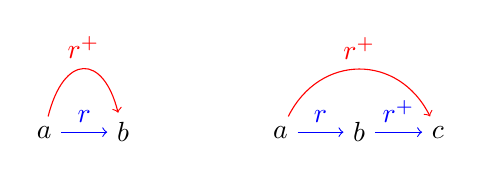
\begin{tikzpicture}
  \node (a0) at (0,0) {$a$};
  \node (b0) at (1,0) {$b$};

  \node (a) at (3,0) {$a$};
  \node (b) at (4,0) {$b$};
  \node (c) at (5,0) {$c$};

  \draw [->,blue] (a0) edge node[above]{$r$} (b0);
  \draw [->,red]
     (a0)
     .. controls (0.25,1) and (0.75,1)
     .. node[above] {$r^+$} (b0);

  \path[->,blue] (a) edge node[above] {$r$} (b);
  \path[->,blue] (b) edge node[above] {$r^+$}    (c);
  \draw[->,red]  (a) .. controls (3.5,1) and (4.5,1) ..  node[above] {$r^+$}  (c);
\end{tikzpicture}


In Alba we write

\begin{alba}
    class
        plus (A:Any) (r: Endorelation A): Endorelation A
            -- 'r.plus' is the transitive closure of 'r'
    :=
        init a b:
            r a b
            => r.plus a b
        step a b c:
            r a b
            => r.plus b c
            => r.plus a c
\end{alba}

The definition uses an inductive type. It has two constructors. The
\code{init} constructor allows us to conclude $r^+ a b$ from $r a b$.  The
\code{step} constructor allows us to conclude $r^+ a c$ from $r a b$ and $r^+
b c$.

By intuition we see that the relation $r^+$ is transitive. But in
order to be sure we need a proof. In order to proof transitivity we have to
prove
%
$$
 r^+ a b \imp r^+ b c \imp r^+ a c
$$
%
for all $a$, $b$ and $c$
i.e. we need a function which looks like
%
\begin{alba}
  f a b c (pab: r.plus a b) (pbc: r.plus b c): r.plus a c :=
    ...
\end{alba}
%
We can do an induction proof on \code{pab: r.plus a b} which generates two
cases.

One case is that \code{r.plus a b} has been constructed
by \code{init a b rab}. In that case we can use the step constructor with
\code{ab: r a b} and \code{pbc: r.plus b c} to construct \code{r.plus a c}.

The second case is that  \code{r.plus a b} has been constructed by \code{step
  a x b (ax: r a x) (pxb: r.plus x b)}. Now we can use the induction
hypothesis to construct from \code{pxb} and \code{pbc} a proof of \code{r.plus
  x c} and then the step constructor to generate a proof of \code{r.plus a c}.


\begin{alba}
    plus_transitive
        (A: Any) (r: Endorelation A)
        : r.plus.is_transitive
    :=
        f a b c (pab: r.plus a b) (pbc: r.plus b c): r.plus a c :=
            inspect
                a; b; pab
            case
                init a b rab :=
                    -- a -> b +> c
                    step a b c rab pbc

                step a x b rax pxb :=
                    {: goal: a -> x +> b +> c
                       by a recursive call to f we prove x +> c
                       and then use the step constructor to prove a +> c :}
                    step a x c rax pxc
                    where
                        pxc: r.plus x c := f x b c pxb pbc
\end{alba}



\subsubsection{Reflexive Transitive Closure}

In the same manner as the transitive closure we can define the reflexive
transitive closure of a relation.

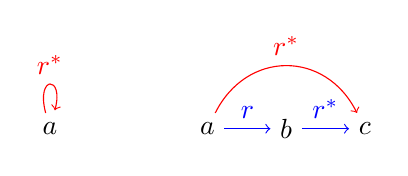
\begin{tikzpicture}
  \node (reflexive) at (0,0) {$a$};
  \node (a) at (2,0) {$a$};
  \node (b) at (3,0) {$b$};
  \node (c) at (4,0) {$c$};

  \path (reflexive) edge [loop above,red] node {$r^*$} (reflexive);

  \path[->,blue] (a) edge node[above] {$r$} (b);
  \path[->,blue] (b) edge node[above] {$r^*$}    (c);
  \draw[->,red]  (a) .. controls (2.5,1) and (3.5,1) ..  node[above] {$r^*$}  (c);
\end{tikzpicture}

\vbox{
\begin{alba}
    class
        star (A:Any) (r: Endorelation A): Endorelation A
          -- 'r.star' is the reflexive transitive closure of 'r'
    :=
        init a:
           r.star a a

        step a b c:
            r a b
            => r.star b c
            => r.star a c
\end{alba}}

Having the definition we prove that the reflexive transitive closure is
transitive.

\begin{alba}
    star_transitive A (r:Endorelation A): r.star.is_transitive :=
        f a b c (sab: r.star a b) (sbc: r.star b c): r.star a c :=
            inspect
                a; b; sab
            case
                init a :=
                    sbc  -- a = b in this case

                step a x b :=
                    step a x c where
                        hypo: r.star x c := f x b c
\end{alba}



\subsubsection{Equivalence Closure}

It is possible to convert any relation into an equivalence relation.

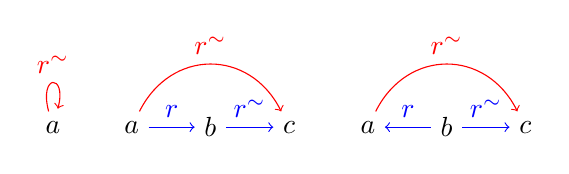
\begin{tikzpicture}
  \node (a0) at (0,0) {$a$};
  \path (a0) edge [loop above,red] node {$r^\sim$} (a0);

  \node (a1) at (1,0) {$a$};
  \node (b1) at (2,0) {$b$};
  \node (c1) at (3,0) {$c$};
  \draw[->,blue] (a1) edge node[above]{$r$} (b1);
  \draw[->,blue] (b1) edge node[above]{$r^\sim$} (c1);
  \draw[->,red] (a1) .. controls (1.5,1) and (2.5,1) .. node [above]{$r^\sim$} (c1);

  \node (a2) at (4,0) {$a$};
  \node (b2) at (5,0) {$b$};
  \node (c2) at (6,0) {$c$};
  \draw[<-,blue] (a2) edge node[above]{$r$} (b2);
  \draw[->,blue] (b2) edge node[above]{$r^\sim$} (c2);
  \draw[->,red]   (a2) .. controls (4.5,1) and (5.5,1) .. node [above]{$r^\sim$} (c2);
\end{tikzpicture}


\begin{alba}
  class
    equivalence A (r: Endorelation A): Endorelation A
  create
    init a:
     r.equivalence a a

    forward a b c:
      r a b => r.equivalence b c => r.equivalence a b

    backward a b c:
      r b a => r.equivalence b c => r.equivalence a b
\end{alba}


The equivalence closure is transitive.

\begin{alba}
  equivalence_is_transitive
    A (r: Endorelation A)
    : r.equivalence.is_transitive :=
    f a b c ab bc: r.equivalence a c :=
      inspect ab case
        forward a x b :=
          forward a x c where
            xc: r.equivalence x c := f x b c

        backward a x b :=
          backward a x c where
            xc: r.equivalence x c := f x b c
\end{alba}

The equivalence closure is symmetric.

\begin{alba}
  equivalence_is_symmetric
    A (r: Endorelation A)
    : r.equivalence.is_symmetric :=
    f a b ab: r.equivalence b a :=
      inspect ab case
        forward a x b :=   -- i.e. 'r a x' is valid
          equivalence_is_transitive r b x a where
            _: r.equivalence b x := f x b
            _: r.equivalence x a := backward x a a
            _: r.equivalence a a := init a

        backward a x b :=  -- i.e. 'r x a' is valid
          equivalence_is_transitive r b x a where
            _: r.equivalence b x := f x b
            _: r.equivalence x a := forward x a a
            _: r.equivalence a a := init a
\end{alba}






\subsection{Diamonds and Confluence}


A relation is a diamond if it is always possible to join two steps with a
single step.

\begin{alba}
  is_diamond A (r: Endorelation A): Proposition :=
      {:   a  ->  b
           |      |
           v      v
           c  -> some d :}
    all a b c:
      r a b
      => r a c
      => some d: r b d and r c d
\end{alba}


A relation is confluent if its reflexive transitive closure is a diamond.

\begin{alba}
  is_confluent A (r: Endorelation A): Proposition :=
    r.star.is_diamond
\end{alba}



We prove that a diamond relation is confluent. Before doing that, we prove a
stripe lemma.

\begin{alba}
  stripe_lemma
    A
    (r: Endorelation A)
    (rdia: r.is_diamond)
    : all a b c:                       --  a *> b
        r.star a b =>                  --  |    |
        r a c =>                       --  v    v
        some d: r b d                  --  c *> d?
                and
                r.star c d :=
     f a b c sab rac :=
       inspect sab case   -- a = b, therefore we use d = c as witness
         init a :=
           _: some d: r a d and r.star c d  where
             _: r.star c c := init c

         step a x b :=
           {:  a  -> x  *> b
               |     |     |
               v     v     v
               c  -> e? *> d? :}
           _ where
             exist_d: some d: r b d and r.star e d := f x b e
             exist_e: some e: r x e and r c e      := rdia a x c
\end{alba}

Then we can prove that a diamond relation is confluent.

\begin{alba}
  diamond_is_confluent
    A
    (r: Endorelation A)
    (rdia: r.is_diamond)
    : r.is_confluent
    :=
      f a b c sab sac: exist d: r.star b d and r.star c d :=
        inspect sab case
          init a :=            -- a = b, therefore we can use d = c
            _ where            --        as witness
              _: r.star b c := sac
              _: r.star c c := init c

          step a x b :=
            {:  a  ->  x  *>  b
                *      *      *
                v      v      v
                c  ->  e? *>  d? :}
            _ where
              exist_d: some d: r.star b d and r.star e d := f x b e
              exist_e: some e: r.star x e and r c e := stripe_lemma r a c x

\end{alba}



\vskip 5mm
\subsection{Transitivity Proofs}

DRAFT: Work with more implicit arguments. Assumption here: All arguments which
can be inferred by the type checker are implicit.



\begin{alba}
    TransitiveRelation (A: Any): Any :=
        Specified (\ (r: Endorelation A) := isTransitive r)

    class
        TransitiveRelation A
    :=
        makeTransitive
            (relation: Endorelation A)
            (transitive:
                all a b c:
                    relation a b => relation b c => relation a c)

    class
        Path A (r: TransitiveRelation A) (a b: A)
    :=
        makePath: r.relation a b -> Path r a b


    (<+>)
        A (r: TransitiveRelation A) a b c
        (p1: Path r a b)
        (p2: Path r b c):
        Path a c
    :=
        inspect p1 case
            makePath rab :=
                inspect p2 case
                    makePath rbc :=
                        inspect r case
                            makeTransitive rel trans :=
                                makePath
                                    (transitive rab rbc)

\end{alba}












\newpage
\section{Lists}
\label{sec:certprog-lists}


In the following we use the definition of the list type from the prelude.

\begin{alba}
  class
    List (A:Any): Any
  create
    [] : List A
    (^): A -> List A -> List A
\end{alba}
%
Note that the operator $\caret$ is right associative and has the
highest precedence of all arithmetic operators.



\subsection{Concatenation}


A standard definition of list concatenation looks like

\begin{alba}
  (+) A (a b: List A): List A :=
    inspect a case
      [] :=
        b
      h ^ t :=
        h ^ (t + b)
\end{alba}
Note that the operator $+$ is left associative.


List concatenation is associative
%
\begin{alba}
  sum_associates A (a b c: List A): a + b + c = a + (b + c) :=
    inspect a case
      h ^ t :=
        goal where
          goal: h ^ t + b + c = h ^ t + (b + c) :=
            via
               h ^ t + b + c
               h ^ (t + b + c)      -- def (+)
               h ^ (t + (b + c))    -- hypo
               h ^ t + (b + c)      -- def (+)
          hypo: t + b + c = t + (b + c) :=
            sum_associates t b c
\end{alba}


\begin{alba}
  nil_right_neutral A (a: List A): a + [] = a :=
    inspect a case
      h ^ t :=
        goal where
          goal: h ^ t + [] = h ^ t :=
            via
              h ^ t + []
              h ^ (t + [])   -- def (+)
              h ^ t          -- hypo
          hypo: t + [] = t :=
            nil_right_neutral t
\end{alba}

Instead of writing the recursive function proving this statement explicitly,
we could use a fixpoint instead.

\begin{alba}
  nil_right_neutral: all A (a: List A): a + [] = a :=
    f A a :=
      inspect a case
        h ^ t :=
          goal where
            goal: h ^ t + [] = h ^ t :=
              via
                h ^ t + []
                h ^ (t + [])   -- def (+)
                h ^ t          -- hypo
            hypo: t + [] = t :=
              f t
\end{alba}



\subsection{Reversal}



A simple function to reverse a list looks like

\begin{alba}
  reverse A (a: List A): List A :=
    inspect a case
      [] :=
        []
      h ^ t :=
        reverse t + [h]
\end{alba}


Next we prove a theorem which shows how reversal and concatenation
interact. Specifically we want to prove
\begin{alba}
  (a + b).reverse = b.reverse + a.reverse
\end{alba}

\begin{alba}
  reversal_of_concatenation
    A
    (a b: List A)
    : (a + b).reverse = b.reverse + a.reverse :=
      inspect a case
        h ^ t :=
          goal where
             goal: reverse (h ^ t + b) = reverse b + reverse (h ^ t) :=
               via
                 h ^ (t + b) |> reverse                     -- def '+'
                 h ^ (reverse b + reverse t) |> reverse     -- hypo
                 (b.reverse + t.reverse) + [h]              -- def 'reverse'
                 b.reverse + (t.reverse + [h])              -- '+' assoc
                 b.reverse + (h ^ t).reverse                -- def 'reverse'

             hypo: (t + b).reverse = b.reverse + t.reverse :=
               reversal_of_concatenation t b
\end{alba}


It is intuitively clear, that a double reversal of a list results in the
original list. We prove this property by
%
\begin{alba}
  double_reversal A (a: List A): a.reverse.reverse = a :=
    inspect a case
      h ^ t :=
        goal where
          goal: (h ^ t).reverse.reverse = h ^ t :=
            via
              (t.reverse + [h]).reverse
              [h].reverse + t.reverse.reverse
              [h] + t
          hypo: t.reverse.reverse = t :=
            double_reversal t
\end{alba}



\subsection{Tail Recursion}

Neither concatenation nor reversal are tail recursive. Furthermore definition
of list reversal is rather inefficient because of the $n^2$
complexity. However we can find equivalent functions which are tail recursive
and efficient.

We need an auxiliary function which reverses a list and prepends it in front
of another list.

\begin{alba}
  reverse_prepend A (a b: List A): List A :=
      -- prepend the reversal of 'a' in front of 'b'
    inspect
      a
    case
      [] :=
        b
      h ^ t :=
        t.reverse_prepend (h ^ b)
\end{alba}


We prove that the function does exactly what we are expecting it to do.

\begin{alba}
  reverse_prepend_correct
    A (a b: List A)
    : a.reverse_prepend b = a.reverse + b :=
      inspect a case
        h ^ t :=
          goal where
            goal: (h ^ t).reverse_prepend  b = (h ^ t).reverse + b :=
              via
                t.reverse_prepend (h ^ b)            -- def
                t.reverse + h ^ b                    -- hypo
                t.reverse + ([h] + b)                -- def '+'
                t.reverse + [h] + b                  -- assoc '+'
                (h ^ t).reverse + b                  -- def 'reverse'
             hypo: t.reverse_prepend (h ^ b) = t.reverse + h ^ b :=
               reverse_prepend_correct t (h ^ b)
\end{alba}


It is obvious that
%
\begin{alba}
  a.reverse_prepend [] = a.reverse
\end{alba}
%
is valid which is a direct consequence of the previous theorem. Alba allows to
override a function definition by an equivalent definition. Therefore we can
substitute the inefficient, non-tail-recursive definition of \code{reverse} by
a more efficient and tail recursive version.

\begin{alba}
  reverse A (a: List A): List A :=
    a.reverse_prepend []
\end{alba}

The definition of list concatenation is efficient, but not tail recursive. By
using the proved theorems we see the following equivalence
%
\begin{alba}
  a + b   =  a.reverse.reverse + b
          =  a.reverse.reverse_prepend b
\end{alba}

Using this, we are able to override the definition of list concatenation by a
tail recursive one

\begin{alba}
  (+) A (a b: List A): List A :=
    a.reverse.reverse_prepend b
\end{alba}

Overriding a definition has no effect during compilation. The original
definition remains to analyze properties. However as soon as the compiler
generates executable code, it replaces the original definition by the
definition which overrides the original definition. It is just an optimization
of the runtime.





\section{Natural Numbers}


The type of natural numbers is defined in the prelude inductively.

\begin{alba}
  class Natural :=
    zero: Natural
    successor: Natural -> Natural
\end{alba}

The number $1$ is the constant

\begin{alba}
  one: Natural := zero.successor
\end{alba}

The compiler \emph{knows} of this type and implements it as an efficient
segmented array to represent arbitrary precision arithmetic. Furthermore all
arithmetic functions like addition, multiplication and relational operators
are implemented as efficient functions. But all these builtin functions behave
as the following functions defined recursively on the inductive type above.



\subsection{Iterators, Recursors and Induction}

\begin{alba}
    iterate (A: Any) (start: A) (step: A -> A): Natural -> A :=
        \ n :=
            inspect n case
                {\ n := A}
                zero        := start
                successor i := step (iterate start step i)

    recurse (A: Any) (start: A) (step: Natural -> A -> A): Natural -> A :=
        \ n :=
            inspect n case
                {\ n := A}
                zero        := start
                successor i := step i (recurse start step i)

    induce
        (F: Natural -> Any)
        (start: F zero)
        (step: all i: F i -> F (successor i)) :
        all n: F n
    :=
        \ n :=
            inspect n case
                {F}
                zero        := start
                successor i := step i (induce start step i)
\end{alba}


Note that only \code{induce} is necessary. We can use \code{induce} to define
the other two functions.

\begin{alba}
    iterate (A: Any) (start: A) (step: A -> A): Natural -> A :=
        induce {\ n := A} start (\ i := step)

    recurse (A: Any) (start: A) (step: Natural -> A -> A): Natural -> A :=
        induce {\ n := A} start step

    -- note:
        (\ n := A) zero ~>  A

        (all i: (\ n := A) i -> (\ n := A) (successor i))
        ~>  all i: A -> A
        =   Natural -> A -> A
\end{alba}







\vskip 5mm
\subsection{Arithmetic}


\subsubsection{Addition}


First we need addition
\begin{alba}
  (+) (a b: Natural): Natural :=
    inspect a case
      0 :=
        b
      n.successor :=
        (n + b).successor
\end{alba}


Addition is associative
%
\begin{alba}
    plusAssociative (a b c: Natural): a + b + c = a + (b + c) :=
        induce
            {\ a := a + b + c = a + (b + c)}

            (identical (b + c))

            (\ n (assoc: n + b + c = n + (b + c)) :=
                apply successor assoc)
            a

    -- Note:
    -- apply (A B: Any) (f: A -> B) {a b: A} (eq: a = b): f a = f b :=
\end{alba}


Now we prove that addition is commutative. In order to prove commutativity of
addition we need two lemmas.

\begin{alba}
    zeroRightNeutral (a: Natural): a + zero = a :=
        induce
            {\a := a + zero = a}

            (identical zero)

            (\ n (neutral: n + zero = n :=
                apply successor neutral)
            a
\end{alba}



\begin{alba}
    pushSuccessor (a b: Natural): successor (a + b) = a + successor b :=
        inspect a case
            zero :=
                identical (successor b)

            successor i :=
                -- goal:
                --   successor (successor i + b) = successor i + successor b
                -- ~>
                --   successor (successor (i + b))
                --   = successor (i + successor b)
                inject _ _
                    (pushSuccessor i b)
                    successor
\end{alba}



\begin{alba}
    plusCommutes (a b: Natural): a + b = b + a :=
        inspect a case
            zero :=
                -- goal: zero + b = b + zero
                -- reduces to: b = b + zero
                zeroRightNeutral b

            successor i :=
                -- goal: successor i + b = b + successor i
                -- ~>    successor (i + b) = b + successor i
                eqTransitive
                    _ _ _
                    (inject _ _ (plusCommutes i b) successor:
                        successor (i + b) = successor (b + i))
                    (pushSuccessor b i:
                        successor (b + i) =  b + successor i)
\end{alba}







\subsubsection{Multiplication}



Multiplication can be defined as a recursive function as well.

\begin{alba}
  (*) (a b: Natural): Natural :=
    inspect a case
        0 :=
            0
        successor i :=
            b + i * b
\end{alba}

\begin{alba}
    zeroRightAbsorber (a: Natural): a * zero = zero :=
        inspect a case
            zero :=
                identical zero

            successor i :=
                -- goal: successor i * zero = zero
                -- ~>    zero + i * zero = zero
                -- ~>    i * zero = zero
                zeroRightAbsorber i
\end{alba}

By substitution is is evident, that $1$ is the left neutral of
multiplication. The number $1$ is right neutral as well, but this assertion
needs a proof.

\begin{alba}
    oneRightNeutral (a: Natural): a * one = a :=
        inspect a case
            zero :=
                identical zero

            successor i :=
                -- goal:  successor i * one = successor i
                -- ~>     one + i * one = successor i
                -- ~>     successor (i * one) = successor i
                inject _ _
                    (oneRightNeutral i)
                    successor
\end{alba}


The distributivity of multiplication over addition is proved by induction.
%
\begin{alba}
    distributeTimes (a b c: Natural): a * (b + c) = a * b + a * c :=
        inspect a case
            zero :=
                identical zero

            successor n :=
                -- goal:  successor n * (b + c)
                --        = successor n * b + successor n * c

                -- ~>     (b + c) + n * (b + c)
                --        = (b + n * b) + (c + n * c)
                eqTransitive _ _ _
                    (inject _ _
                        (distributeTimes n b c)
                        (\ x := (b + c) + x)
                        : (b + c) + n * (b + c) = (b + c) + (n * b + n * c))
                    reorder b c (n * b) (n * c)
                where
                    reorder b c x y: (b + c) + x + y = (b + x) + (c + y)
                    :=
                        -- reordering manually is very tedious
                        -- must invent some compiler support
                        ??
\end{alba}

Commutativity of multiplication can be proved by using distributivity.

\begin{alba}
  times_is_commutative (a b: Natural): a * b = b * a :=
    inspect a case
      0 :=
       via 0 * b
           0
           b * 0
       where
         _: b * 0 = 0 := times_zero_is_zero b

      1 + n :=
        via
          (1 + n) * b
          b + n * b
          b + b * n
          b * 1 + b * n
          b * (1 + n)
        where
          hypo: n * b = b * n := times_is_commutative n b
          _: b * 1 + b * n := times_is_distributive b a n
\end{alba}






\subsection{Order Relation}

We define the order relation on natural numbers inductively.

\begin{alba}
    class
        (<=): Endorelation Natural
    :=
        init n:
            0 <= n

        step n m:
            n <= m
            => n.successor <= m.successor
\end{alba}
%
Note that in \code{init n} the argument \code{n} is implicit and in \code{step n
m ...} the arguments \code{n m} are implicit.

We can generate an induction law.
\begin{alba}
    leInduction
        (r: Endorelation Natural)
        (ini: all i: r 0 i)
        (stp: all i j: r i j => r i.successor j.successor)
        : all i j: i <= j => r i j
    :=
        \ i j le :=
            inspect le case
                init: ini
                step le0 := stp (leInduction ini stp le0)
\end{alba}

The inductive type has no parameters and two index arguments. The index
arguments are of type \code{Natural}. Therefore the compiler can do some analysis
on the pattern which can constitute the proposition \code{n <= m}

\begin{alba}
        n               m                   constructor

        0               0                   init 0

        0               j.successor         init j.successor

        i.successor     0                   impossible

        i.successor     j.successor         step i j iLEj
\end{alba}
%
Using this analysis the compiler generates the following propositions
\begin{alba}
    discriminate: all n: not n.successor <= 0

    inversion: all n m: n.successor <= m.successor => n <= m
\end{alba}

Let's do the proofs by hand.

\begin{alba}
    discriminate (n: Natural): n.successor <= 0 => false :=
        leInduction
            {\ n m :=
                inspect n case
                    zero := true
                    i.successsor :=
                        inspect m case
                            zero := false
                            j.successor := true}
            (\ m := trueValid)
            (\ n m le := trueValid)

    discriminate {n: Natural} (le: n.successor <= 0): false :=
        inspect
            n.successor
            0
            le
        case
            {\j k le :=
                inspect j case
                    zero := true -- match for 'init'
                    n.successor :=
                        inspect k case
                            zero := false       -- match for 'inspect'
                            m.successor := true -- match for 'step'
            }
            init k :=
                trueValid
            step n m le :=
                trueValid

    invert {n m: Natural} (le: n.successor <= m.successor): n <= m
    :=
        inspect
            n.successor
            m.successor
            le
        case
            {\ j k le :=
                inspect j case
                    zero := true  -- match for 'init'
                    n.successor :=
                        inspect k case
                            zero := true    -- not used
                            m.successor :=  -- match for 'step' and 'inspect'
                                n <= m}
            init k :=
                trueValid

            step n m le :=
                le
\end{alba}

\begin{alba}
    leZeroIsZero (a: Natural): a <= 0 => a = 0 :=
        inspect a case
            zero :=
                \ le := identical zero
            n.successor :=
                discriminate {n} >> exFalso
\end{alba}





\noindent The order relation is reflexive i.e. $a \le a$.

\begin{alba}
    reflexive: (a: Natural): a <= a :=
        inspect a case
            zero :=
                init 0
            n.successor :=
                step n n (reflexive n)
\end{alba}


\begin{alba}
    -- other proof of reflexivity
    reflexive (a: Natural): a <= a :=
        natInduction init step a

    -- Induction predicate
    -- f a := a <= a

    -- 'init' proves 'f zero' i.e. 'zero <= zero'
    -- 'step' proves 'all i: f i -> f i.successor'
    --     i.e. 'i <= i => i.successor <= i.successor
    --     with implicit argument 'i'
\end{alba}



\noindent Next we prove the law $a \le b \imp a \le 1 + b$.

\begin{alba}
    leImpliesLeSucc
        (a b: Natural)
        :  a <= b  =>  a <= b.successor
    :=
        case
            init b :=
                init b.successor

            step n m lenm :=
                -- a = n.successor, b = m.successor
                -- goal: n.successor <= m.successor.successor
                step
                    n
                    m.successor
                    (leImpliesLeSucc n m lenm)
\end{alba}


We can define an induction law for $\le$.

\begin{alba}
    induceLe
        (r: Endorelation Natural)
        (ini: all m: r zero m)
        (stp: all j k: r j k => r j.successor k.successor)
        (n m: Natural)
        (le: n <= m)
        : r n m
    :=
        inspect n m le case
            init m :=
                ini m
            step j k jk :=
                stp j k (induceLe r ini stp j k jk)
\end{alba}


\noindent The strict order relation $<$ is defined as

\begin{alba}
  (<) (a b: Natural): Proposition :=
    successor a <= b
\end{alba}

Properties:

\begin{alba}
    leToLt: (a b: Natural) (le: a <= b): a /= b => a < b :=
        inspect le case
            init b: 0 /= b => 0 < b :=
                inspect b case
                    zero: \ ne := identical zero |> ne |> exFalso
                    successor i: 0 /= successor i => 0 < successor i :=
                        \ ne := step (init i)
            step i j ij
            : successor i /= successor j => successor i < successor j :=
                \ ne :=
                    step (leToLt ij (ne << apply successor))
\end{alba}






\vskip 5mm
\section{Decision Procedure for the Order Relation}

A decision between two alternatives is an inductive type.

\begin{alba}
    class Decision2 (a b: Proposition): Any :=
        left: a  -> Decision2 a b
        right: b -> Decision2 a b

    Decision (a: Proposition): Any :=
        Decision2 a (not a)
\end{alba}



\begin{alba}
    (<=): all (a b: Natural): Decision (a <= b) :=
        \ a :=
            inspect a case
                zero :=
                    left << init
                successor i :=
                    \ b :=
                        inspect b case
                            {\ b := Decision (successor i <= b)}
                            zero :=
                                right discriminate
                            successor k :=
                                mapDecision (i <= k)
        where
            mapDecision
                {i j} (d: Decision (i <= j))
                : Decision (successor i <= successor j)
            :=
                inspect d case
                    left le0 :=
                        left (step le0)
                    right nle0 :=
                        right (nle0 << invert)
\end{alba}





\vskip 5mm
\section{Search}

\begin{alba}
    Decider (A: Any) (f: Predicate A): Any :=
        all x: Decision (f x)

    class StrongMaybe (A: Any) (f: Predicate A) (a: Proposition): Any :=
        just x: f x -> StrongMaybe f a
        nothing: a -> StrongMaybe f a

    lowerBound (f: Predicate Natural) (n: Natural): Proposition :=
            -- 'n' is a lower bound for all numbers which satisfy 'f'.
        all i: f i => n <= i

    least (f: Predicate Natural) (n: Natural): Proposition :=
            -- 'n' is the least number which satisfies 'f'
        lowerBound f n and f n

    nextLowerBound
        (f: Predicate Natural) (n: Natural)
        (lb: lowerBound f n) (nfn: not (f n))
        : lowerBound f (successor n)
    :=
        \ i fi: successor n <= i :=
            inspect n = i case
                left eq :=
                    fi |> leibniz eq nfn
                right neq :=
                    leToLt lb neq

    findBelow
        (f: Predicate Natural)
        (d: Decider f)
        (bound: Natural)
        : StrongMaybe (least f) (lowerBound f bound)
    :=
        search 0 bound (identical bound) (\ i e := init i)
        where
            search
                i k
                (inv1: bound = i + k)
                (inv2: lowerBound f i)
                : StrongMaybe f (lowerBound f i)
            :=
                inspect k case
                    zero :=
                        nothing inv2
                    successor j :=
                        inspect d i case
                            left sat :=
                                just i (inv2,sat)
                            right notsat :=
                                search
                                    i.successor
                                    j
                                    (leibniz
                                        {(=) bound}
                                        inv1
                                        (pushSuccessor {i} {j} |> flip)
                                    (nextLowerBound inv2 notsat)
\end{alba}




\begin{alba}
    find
        (f: Predicate Natural)
        (d: Decider f)
        (e: exist f)        -- There is some number satisfying 'f'
        : Refined (least f)
    :=
        MISSING
\end{alba}



\vskip 5mm
\section{Properties of Constructors of Inductive Types}

There are two properties of constructors of inductive types which are very
important and valid for all inductive types.

\begin{enumerate}

\item Constructors are unique: Objects constructed by
different constructors are different.

\item Constructors are injective: Equal objects constructed by the same
constructor must have been constructed by applying the constructor to the same
arguments.

\end{enumerate}

We prove these properties for natural numbers. The proofs for other constructors
of other inductive types follow the same pattern.




\subsection{Uniqueness of Constructors}

In order to prove the uniqueness of the constructors of natural numbers we have
to prove the proposition

\begin{alba}
    all (n: Natural): 0 /= n.successor
\end{alba}

Remember that \code{0 /= n.successor} is equivalent to \code{0 = n.successor =>
false}. In order to prove the property we have to find a function which
maps any natural number \code{n} and a proof of \code{0 = n.successor} into a
proof of \code{false}.

Since we can assume \code{0 = n.successor} we can use the leibniz property that
\code{0} and \code{n.successor} satisfy the same predicates. If we find a
predicate over natural numbers which we can prove for \code{0} we can use the
leibniz rule to prove that \code{n.successor} satisfies the same predicate.

We use the predicate
\begin{alba}
    f: Natural -> Proposition :=
        case
            0 :=
                true
            k.successor :=
                false
\end{alba}

Evidently \code{f 0} and \code{true} are equivalent propositions and \code{f
n.successor} and \code{false} are equivalent propositions.

A proof of \code{f 0} i.e. \code{true} is trivial, because the proposition
\code{true} is an inductive type with one constructor.

\begin{alba}
    class true: Proposition := trueValid
\end{alba}


Here is the complete proof of the mutual exclusivity of the two constructors of
natural numbers.


\begin{alba}
    discriminate (n: Natural): 0 /= n.successor
    :=
        (\ (eq: 0 = n.successor): false := g n.successor eq)
        where
            g: all k: 0 = k => f k :=
                case
                    identical :=
                        -- goal: f 0
                        trueValid
            f :=
                case 0 := true; k.successor := false
\end{alba}


There is an alternative way to write \code{discriminate} with an elimination
function

\begin{alba}
    discriminate (n: Natural): 0 /= n.successor :=
        \ (eq: 0 = n.successor) :=
            inspect
                n.successor     -- index (optional, can be ommitted)
                eq              -- inductive object
            case
                {\ i p :=
                    inspect i case
                        zero := true
                        successor k := false}
                identical := trueValid
\end{alba}

Instead of \code{true} we could use \code{all (A: Proposition):A -> A} and
prove it by \code{\mybackslash\ A x := x} instead of \code{trueValid}.




\subsection{Injectivity of Constructors}

The injectivity of the successor function of natural numbers can be expressed
by the property

\begin{alba}
    all (n m: Natural): n.successor = m.successor  =>  n = m
\end{alba}

In order to prove this property we need only a little trick. We have to
express the goal \code{n = m} as a function of variable representing the right
hand side of the premise equality which returns the required goal, when
instantiated with \code{m.successor}. It might not be trivial to find such a
function, but it is easy to see that the following function does the job.

\begin{alba}
    f: Natural -> Proposition :=
        case 0 :=
                true
             i.successor :=
                n = i
\end{alba}
%
Having that function the actual proof is a straightforward pattern match on the
premise equality.


\begin{alba}
    invert (n m: Natural) (eq: n.successor = m.successor): n = m
    :=
        g m.successor eq
        where
            g: all k: n.successor = k => f k :=
                case identical :=
                    -- goal f n.successor
                    identical
            f :=
                case
                    0 :=
                        true -- never used
                    i.successor :=
                        n = i
\end{alba}


We can write \code{invert} as well with an elimination function

\begin{alba}
    invert (n m: Natural) (eq: n.successor = m.successor): n = m :=
        inspect
            m.successor
            eq
        case
            {\ i p :=
                inspect i case
                    zero :=
                        true -- not used
                    successor m :=
                        n = m}
            identical :=
                identical n
\end{alba}

Note that for the matching case the elimination function is called with the
arguments \code{n.successor} and \code{eq} and returns \code{n=n}.  This is
correctly proved by \code{identical n}.

However for the whole pattern match the elimination function is called with the
arguments \code{m.successor} and \code{eq} and returns \code{n = m}. I.e. the
whole inspect expression returns a proof of \code{n = m}.







\subsection{Types with Indices}

Consider the inductive predicate

\begin{alba}
    class
        isEven: Predicate Natural
    :=
        zero: isEven 0
        next: all n: isEven n => isEven n.successor.successor
\end{alba}

The proposition \code{isEven 0} can be constructed only with the first
constructor. The proposition \code{isEven k.successor.successor} can be
constructed only with the second constructor. We can make a further case split
on \code{k}.  \code{isEven 0.successor} is impossible to construct and
\code{isEven n.successor.successor} implies \code{isEven n}.

I.e. we should be able to prove the following propositions:

\begin{alba}
    discriminate: not 0.successor.isEven

    invert: all n: isEven n.successor.successor => isEven n
\end{alba}


\noindent First we prove \code{discriminate}
%
\begin{alba}
    discriminate: not 0.successor.isEven
    :=
        g 0.successor
        where
            g: all k: k.isEven => f k :=
                case
                    zero :=
                        -- goal: f 0
                        trueValid
                    next n evN :=
                        -- goal: f n.successor.successor
                        trueValid
            f: Predicate Natural :=
                case
                    0 :=
                        true
                    m.successor :=
                        inspect m case
                            0 :=
                                false
                            _.successor :=
                                true
\end{alba}




\noindent Now we prove \code{invert}
%
\begin{alba}
    invert (n: Natural): n.successor.successor.isEven => n.isEven
    :=
        g n.sucessor.successor
        where
            g: all k: k.isEven => f k :=
                case
                    zero :=
                        -- goal: f 0
                        trueValid
                    next m evM :=
                        -- goal: f m.successor.successor
                        evM
            f: Predicate Natural :=
                case
                    0 :=
                        true
                    k.successor :=
                        inspect k case
                            0 :=
                                true -- never used
                            m.successor :=
                                m.isEven
\end{alba}




\noindent NEEDS REWORK WITH NEW DEPENDENT PATTERN MATCH

These proofs create a lot of overhead. Some compiler support shall be available
to them in a simpler manner.

First let's look at the proof of
\begin{alba}
    discriminate: isEven 0.successor => false :=
        case ...
\end{alba}
The pattern matches a proof of \code{isEven 0.successor} against the two
possible constructors
\begin{alba}
    zero: isEven 0
    next n: isEven n => isEven n.successor.successor
\end{alba}
First the compiler tries to the premise with the final types of the
constructors.
\begin{alba}
    -- Needed unifications
    isEven 0.successor              isEven 0
    isEven 0.successor              isEven n.successor.successor
\end{alba}
Both unifications fail. I.e. a proof of \code{isEven 0.successor} cannot be
generated by none of the two constructors. Note that a failure of the
unification always comes from a failure to unify the indices. \code{isEven} is
an indexed type, indexed by a natural number. The failure to unify comes from
the fact, that the typed to be pattern matched has indices which are not
variables.

Since both unifications fail, both branches can be ommitted from the source code
and the compiler can generate the cases internally. In order to do that, it has
to generate a proper elimination function. An elimination function for an
indexed inductive type $T$ has the form
$$
    \lambda \ybold^\Bbold x^{T \ybold}. R
$$
It has $n + 1$ arguments where $n$ is the number of indices. $\ybold$ is the
array of indices and $x$ is a bound variable representing the expression to be
pattern matched on.

In our case the argument $x$ is irrelevant. The elimination function has to
return the goal \code{false} for the index argument \code{0.successor} and
something with a trivial proof for all the other cases (e.g. \code{goal -> goal}
which is provable by the identity function. As long as primitive values of an
inductive type are involved, such a elimination function can be generated by the
compiler in case of a failed unification.

The type checker is happy, because it has for each case a term is of the
appropriate type for the branch and the overall goal is satisfied as well.

A complete pedantic proof with an explicitely entered elimnation function looks
like
\begin{alba}
    discriminate isEven 0.successor => false :=
        \ ev := g 0 ev where
            g k ev :=
                inspect
                    ev
                    \ j p := inspect j case
                        0 := false => false
                        m.succ :=
                            inspect m case
                                0 := false
                                n.succ := false => false
                case
                    zero :=
                        identity
                    next i p :=
                        identity
\end{alba}
But the shorter one should do its job as well.
\begin{alba}
    discriminate isEven 0.successor => false :=
        case --  <--- no valid cases to analyze
\end{alba}

\vskip 5mm
Now let's look at the proof of

\begin{alba}
    inversion k: isEven k.successor.successor => isEven k :=
        case ...

    -- needed unifications
    isEven k.successor.successor        isEven 0
    isEven k.successor.successor        isEven n.successor.successor
\end{alba}
The first one fails and the second one unifies $k$ with $n$.




\vskip 5mm
Now let's look at a definition of the even and odd property of natural numbers
defined as a mutual type family.
%
\begin{alba}
    mutual
        class
            isEven: Natural -> Proposition
        :=
            zero: isEven 0

            fromOdd n: n.isOdd => n.successor.isEven

        class
            isOdd: Natural -> Proposition
        :=
            fromEven n: n.isEven => n.successor.isOdd
\end{alba}
%
Looking at the possible ways to construct the even or the odd property we should
be able to proof the following theorems.
%
\begin{alba}
    discriminate: not 0.isOdd

    invertEven n: n.successor.isEven => n.isOdd

    invertOdd  n: n.successor.isOdd  => n.isEven
\end{alba}


\noindent We prove the properties one by one.

\begin{alba}
    discriminate: not 0.isOdd :=
        (\ odd := f 0 odd identical)
        where
        f n: n.isOdd => 0 = n => false
        :=
            case
                fromEven k _ :=
                    -- goal: 0 = k.successor => false
                    discriminate

    invertEven n: n.successor.isEven => n.isOdd
    :=
        (\ ev := f n.successor ev identical)
        where
        f k: k.isEven => k = n.successor => n.isOdd
        :=
            case
                zero :=
                    -- goal 0 = n.successor => false
                    discriminate n

                fromOdd m mOdd :=
                    -- goal: m.successor = n.successor => n.isOdd
                    invert m n -- produces m = n
                    >>
                    case
                        identical := mOdd

    invertOdd n: n.successor.isOdd => n.isEven
    :=
        (\ odd := f n.successor odd identical)
        where
        f k: k.isOdd => k = n.successor => n.isEven
        :=
            case
                fromEven m mEven :=
                    -- goal: m.successor = n.successor => n.isEven
                    invert m n -- produces m = n
                    >>
                    case
                        identical := mEven
\end{alba}

The trick to prove these kind of properties is always the same. Whenever we have
a goal or a premise of a special form like \code{0.isOdd} or
\code{m.successor.isOdd} we replace the special term by a variable to get
\code{n.isOdd} and introduce an equality like \code{0 = n} or \code{n =
m.successor} to have an equivalent formulation.

With the variable we can do a pattern match and use a further pattern match on
the corresponding equality or a discrimination to prove the goal.

Once the trick has been understood, it is a fairly mechanical excercise. Since
this a repetitive task for all newly defined inductive propositions, it is
better to let the compiler derive the corresponding inversion and discrimination
properties.



\subsection{Compiler Generated Proofs Involving Constructors}



\begin{alba}
    reject (n: Natural): 0 = n.successor => false
    :=
        (\ k :=
            (case identical := trueValid)
            : 0 = k
              =>
              (case 0 := true; _.successor := false) k)
          n.successor
\end{alba}


\begin{alba}
\end{alba}





\section{Vectors}


FOR DISCUSSION!!


Vectors or length indexed lists are an often used example to show dependent
types. A vector in Alba can be defined as

\begin{alba}
    class
        Vector (A: Any): Natural -> Any
    :=
        nil: Vector A 0

        cons: all n: A -> Vector A n -> Vector A n.successor
\end{alba}

Due to the current conventions such a type is a little bit clumsy in Alba,
because \code{n} is not an implicit argument, i.e. one cannot construct a vector
with
%
\begin{alba}
    cons 'A' <| cons 'B' <| nil  -- Invalid!!
\end{alba}
%
%
Instead we have to write

\begin{alba}
    cons 1 'A' <| cons 0 'B' <| nil: Vector Character 2
\end{alba}


We can append two vectors.

\begin{alba}
    append
        (A: Any) (n m: Natural):
        Vector A n -> Vector A m -> Vector A (n + m)
    :=
        case
            nil :=
                identity

            cons k e v :=
                \w :=
                    cons (k + m) e <| append k m v w
\end{alba}


\begin{alba}
    reverse (A: Any) (n: Natural): Vector A n -> Vector A n
    :=
        case
            nil :=
                nil

            cons k e v :=
                append
                    (reverse k v)
                    (cons 0 e nil)

    -- Note: This function does not typecheck. The append function returns
    --       an object of type 'Vector A (k + 0.successor)' while it
    --       should return an object of type 'Vector A (0.successor + k)'
    -- A proof would be necessary to show that both types are identical.
\end{alba}


This example shows that dependent types like \code{Vector} are not very usable
in practice. Usually computational objects should not have a dependent type. If
we want to specify that a type has a certain property, a good option is to use
\code{Specified} which allows to extract the object and the proof and tread them
separately.

\noindent E.g. we could use
\begin{alba}
    Specified (\ (l: List A) := length l = n)
\end{alba}
%
to specify a list with a certain length. The \code{value} and \code{proof}
functions allow the extraction of the list and the proof of the property.






\section{Red Black Trees}

Ideas from Stephanie Weyrich's Haskell implementation:

\begin{alba}
    class Color := red; black

    class height: Proposition := zero: height; succ: height -> height


    incr (c: Color) (h: height): height :=
        inspect c case
            red := h
            black := succ h

    class
        RBT A: Color -> height -> Any
    :=
        nil: RBT A black zero

        tr h c1 c2: RBT A c1 h -> A -> RBT A c2 h -> RBT A black (succ h)

        tb h: RBT A black h -> A -> RBT A black h -> RBT A red h


    class
        Almost A: height -> Any
    :=
        almost h c1 c2 c: RBT c1 h -> A -> RBT c2 h -> Almost (incr c h)

    class
        Hidden A: height -> Any
    :=
        hr h: RBT red h -> Hidden h

        hb h: RBT black (succ h) -> Hidden (succ h)
\end{alba}











%%% Local Variables:
%%% mode: latex
%%% TeX-master: "main_alba_design"
%%% End:
